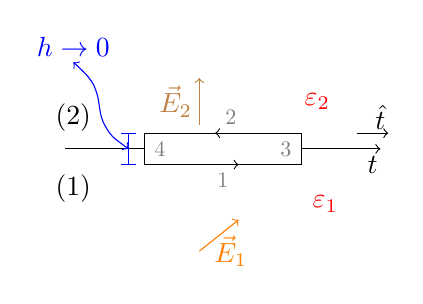
\begin{tikzpicture}

\draw (0,0) -- (1,0);
\draw [->,] (3,0) -- (4,0);
\draw  (1,0.2) rectangle (3,-0.2);
\node at (0.1,-0.5) {$(1)$};
\node at (0.1,0.4) {$(2)$};
\node at (3.3,-0.7) [red]{$\varepsilon_1$};
\node at (3.2,0.6) [red]{$\varepsilon_2$};
\node at (3.9,-0.2) {$t$};
\draw [->,] (3.7,0.2) -- (4.1,0.2);
\node at (4,0.4) {$\hat{t}$};
\draw [|-|, blue] (0.8,0.2) -- (0.8,-0.2);
\draw [->,orange] (1.7,-1.3) -- (2.2,-0.9);
\draw [->,brown] (1.7,0.3) -- (1.7,0.9);
\node at (1.4,0.6) [brown] {$\vec{E}_2$};
\node at (2.1,-1.3)  [orange]{$\vec{E}_1$};
\draw [<->,blue] plot[smooth, tension=.7] coordinates {(0.8,0) (0.5,0.3) (0.4,0.7) (0.3,0.9) (0.1,1.1)};
\node at (0.1,1.3) [blue]{$h\rightarrow0$};
\draw [->] (1.8,-0.2) -- (2.2,-0.2);
\draw [->] (2.3,0.2) -- (1.9,0.2);
\node [scale=0.8, gray] at (2,-0.4) {$1$};
\node [scale=0.8, gray] at (2.1,0.4) {$2$};
\node [scale=0.8, gray] at (2.8,0) {$3$};
\node at (1.2,0) [scale=0.8, gray]{$4$};
\end{tikzpicture}